\chapter{Wireless Sharing and Access Control}\label{waccess}\index{Access control}

\minitoc 

\clearpage
\section*{Objectives}
To develop 
\begin{itemize}

\item 

\item 

\item 

\item 

\end{itemize}

\section{Carrier Sense Multiple Access (with Collision Avoidance)}\index{CSMA/CA}

Carrier-sense multiple access with collision avoidance (CSMA/CA) is a
medium access control protocol developed for IEEE 802.11 wireless local
area networks.  This method is used to assist with collision avoidance
in wireless networks, where multiple wireless devices connected to the
wireless network can "see" access points forming part of the wireless
network but not other wireless devices.

In early versions of wired Ethernet networks adopted the carrier-sense
multiple access with collision detection (CSMA/CD) protocol to allow the
orderly transmission of data across the network. In wireless networks, it
is harder for a device to detect collisions taking place so a prevention
(avoidance) method is adopted which aims to prevent any collisions
happening in the first place.

Some of the reasons for the difficulty in detecting collisions include
differences in transmit power level, the receive sensitivity, the
range and location of the device with respect to the access point. These
factors may cause an access point to not be able to "hear" another access
point's broadcast. This condition in a wireless network is referred to as
"hidden node".

The high level sequence of hand shakes between the device and the access
point takes place when a device is  prepared to send data over a wireless
network, with CSMA/CA capability enabled. The communication hand shaking
between the device and access point include:

\begin{enumerate}[(i)]

\item When a device is about to send data, it check that the communications 
channel is "idle" and sends out a request to send (RTS)\index{RTS} message to the "seen" access point/s.
\item The access point receives the RTS message and if there's no other 
simultaneous data communications taking place by other connected devices, 
it sends the device a clear to send (CTS)\index{CTS} message.
\item In the case the access point receives the RTS message and simultaneous 
data communications is taking place between other devices (ie; risk of collision 
exists), then no CTS message is sent to the waiting device.
\item After a randomly wait time generated by the device lapses, the 
device will re-send the RTS to the access point/s.
\item This process is repeated until a free communications channel is 
available and a CTS message is received from the access point.

\end{enumerate}

\begin{figure}
\centering
	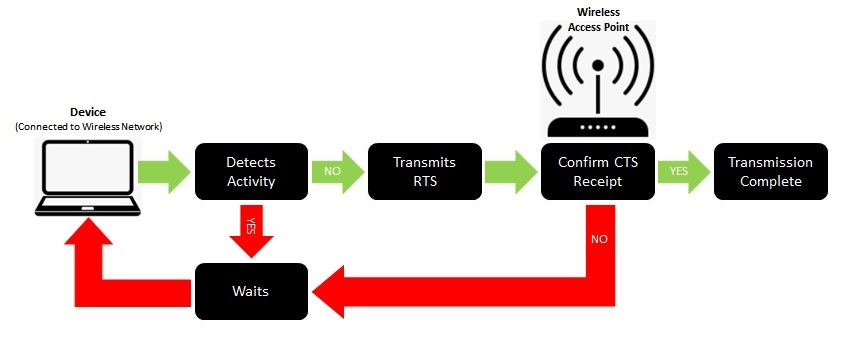
\includegraphics[width=12cm]{CSMA_CA}
	\caption{CSMA/CA Data Message Transmission Process}
	\label{CSMA_CA}
\end{figure}


\section{Sharing by Treating Other Channels as Noise}

\section{Other Methods of Access Sharing}

\subsection{Code Sharing}\index{code sharing}

\subsection{OFDMA}\index{OFDMA}
